\chapter{Concepción y dise\~no de la solución}\label{chapter:proposal}

%En este capítulo, se aborda el desafío de concebir y diseñar la metodología propuesta para superar limitaciones en los modelos de tópicos. Se enfrentan dos obstáculos clave: la automatización de la estimación del número óptimo de tópicos y la asignación autónoma de nombres a dichos tópicos.
%
%La estructura del capítulo se organiza en dos fases esenciales: el Pre-Procesamiento Semántico y la Recuperación por Tópicos. En la primera fase, se explora a fondo cada etapa del Pre-Procesamiento Semántico, desde el procesamiento léxico hasta el descubrimiento de tópicos mediante el algoritmo Latent Dirichlet Allocation (LDA). Se destaca una estrategia innovadora para la identificación automática del número de tópicos, basada en un algoritmo de clustering autoincremental que elimina la necesidad de estimaciones previas por expertos. Asimismo, se presenta un método para asignar nombres significativos a los tópicos, enriqueciendo la comprensión semántica de los resultados. En la segunda fase, denominada Recuperación por Tópicos, se aborda la concepción de un motor de búsqueda diseñado para aprovechar las ventajas obtenidas en la fase anterior. Este motor busca no solo eficiencia en la recuperación de información sino también una presentación ordenada y contextualizada de los resultados, guiada por la estructura temática identificada previamente.

Este capítulo explora la arquitectura esencial del programa, centrando su atención en el trayecto desde el Pre-procesamiento Sem\'antico hasta la Recuperación de Informaci\'on por Tópicos. La Figura 2.1 actúa como guía visual para estas dos etapas.

Se inicia con un preprocesamiento léxico básico, estructurando el texto para las operaciones subsiguientes. La Identificación de la Cantidad de Tópicos adopta un enfoque de agrupación semántica y embeddings, eliminando la necesidad de intervención de expertos para obtener información sobre la distribución del corpus. Esta fase se entrelaza con el modelo de Latent Dirichlet Allocation (LDA) para desentrañar patrones temáticos. La transición hacia la Asignación de Nombres a Tópicos conecta el descubrimiento de tópicos con una ontología de dominio general, seleccionando palabras clave basadas en las probabilidades de LDA. Esta estrategia busca facilitar una asignación contextualizada de nombres.

En pos de aplicación y visualización, se implementa un motor de búsqueda que, al recibir una consulta, devuelve resultados organizados según su relevancia y tópicos (nombrados) asociados, permitiendo una exploración más interpretable.

A través de este recorrido, la arquitectura del programa se presenta como una combinación de componentes interconectados, cada uno contribuyendo a la extracción y comprensión de información significativa de conjuntos de datos textuales.

\begin{figure}[H]
	\centering
	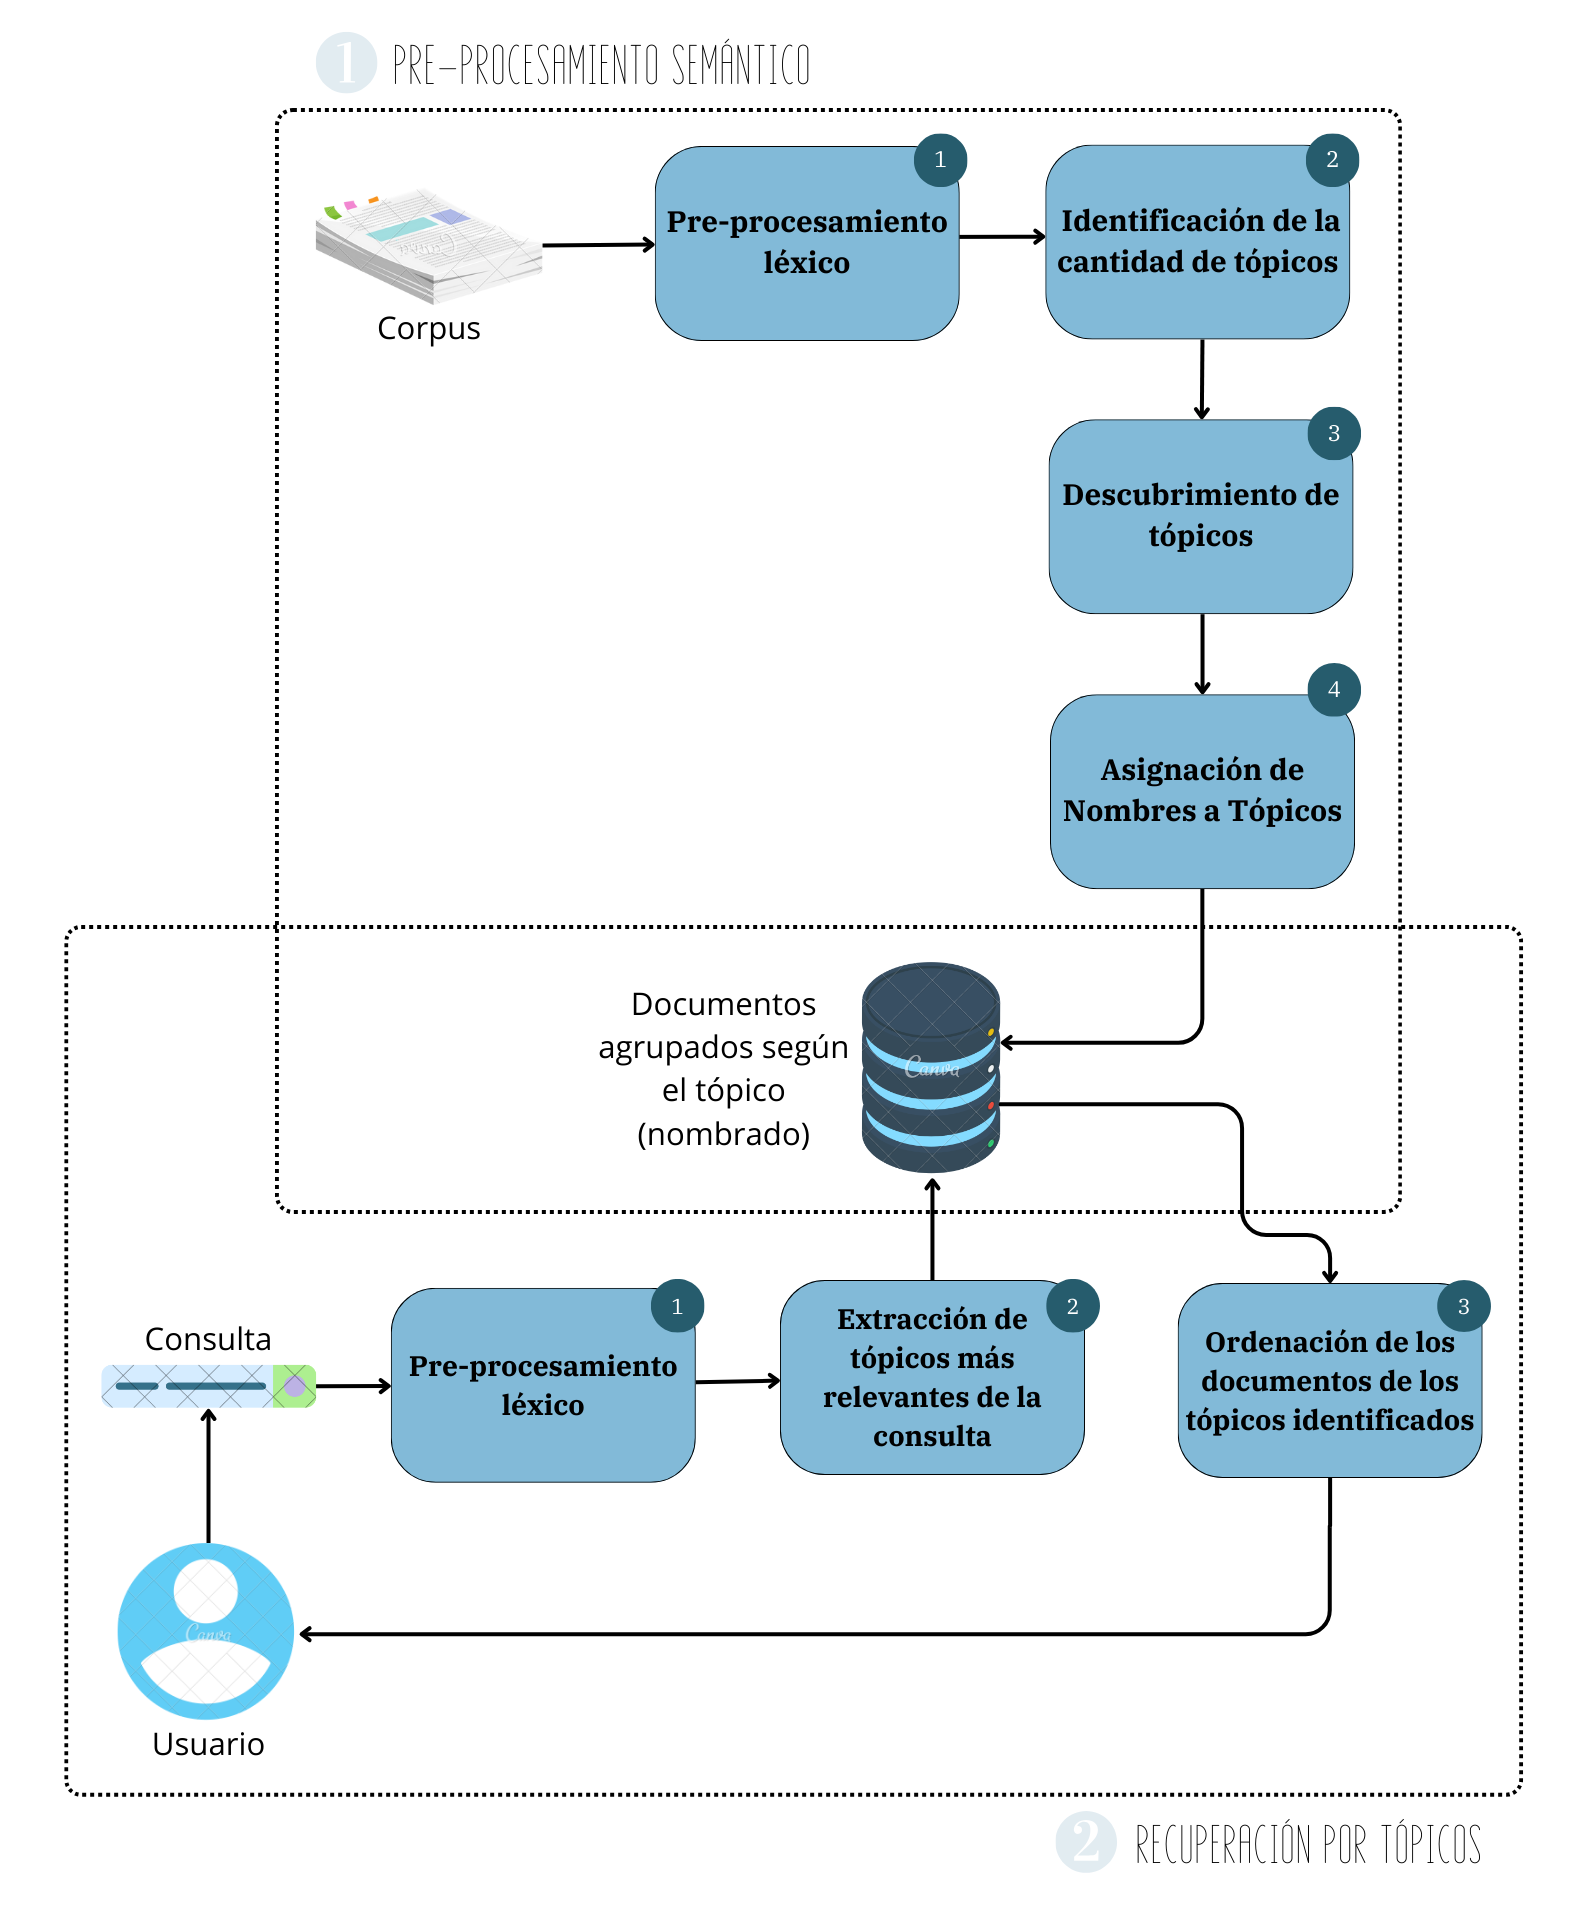
\includegraphics[width=15cm]{Architecture.png}
	\caption{Arquitectura del sistema}
\end{figure}

\newpage
\section{Pre-procesamiento sem\'antico}

En la búsqueda constante por perfeccionar los modelos de tópicos en el procesamiento de texto, esta secci\'on se enfoca en dos aspectos cruciales: la estimación automática del número de tópicos antes de la aplicación del modelo y la asignación automática de nombres a los tópicos identificados. Estos elementos desempeñan un papel fundamental en la mejora de la interpretación y utilidad de los resultados obtenidos mediante técnicas como Latent Dirichlet Allocation (LDA). La automatización de estos procesos no solo simplifica la implementación de modelos, sino que también enriquece la comprensión de patrones temáticos en grandes conjuntos de datos textuales, allanando el camino hacia un análisis más eficiente y accesible.

\subsection{Pre-procesamiento l\'exico}

En el ámbito del procesamiento de texto, el preprocesamiento léxico desempeña un papel fundamental al garantizar la adecuada preparación del texto antes de su análisis. Este proceso es esencial en cualquier sistema de procesamiento de texto, ya que establece las bases para la comprensión y extracción de información significativa. En este contexto, se sigue un preprocesamiento léxico básico (ver figura 2.2), un conjunto de pasos iniciales que buscan homogeneizar y organizar el texto de manera que facilite las tareas posteriores de análisis y procesamiento. 

La primera etapa del preprocesamiento léxico comienza con la tokenización, fragmentando el texto en unidades léxicas para facilitar la identificación y manipulación de palabras. Seguidamente, se lleva a cabo la eliminación de ruido, suprimiendo elementos redundantes como signos de puntuación o números, que podrían interferir con la interpretación precisa del contenido. A continuación, se realiza la exclusión de términos comunes que carecen de relevancia semántica significativa. 

Para la reducción morfológica del vocabulario existen dos t\'ecnicas: lemmatizaci\'on y stemming. La lematización simplifica la identificación de términos al reducir las palabras a sus formas base, mientras que el stemming halla formas truncadas al eliminar sufijos y prefijos. Se escoge la lematizaci\'on debido al requisito de trabajar con palabras reales para modelos y ontologías en nuestro contexto específico, cosa no garantizada en el stemming. Posteriormente, se aplica un filtrado según la ocurrencia, eliminando términos poco frecuentes o excesivamente repetitivos. 

Se construye el vocabulario del corpus y se representan vectorialmente los documentos, eligiendo en este estudio específicamente la representación de bolsa de palabras. Además, se elabora la matriz de co-ocurrencia de términos para capturar las correlaciones entre palabras.

\begin{figure}[H]
	\centering
	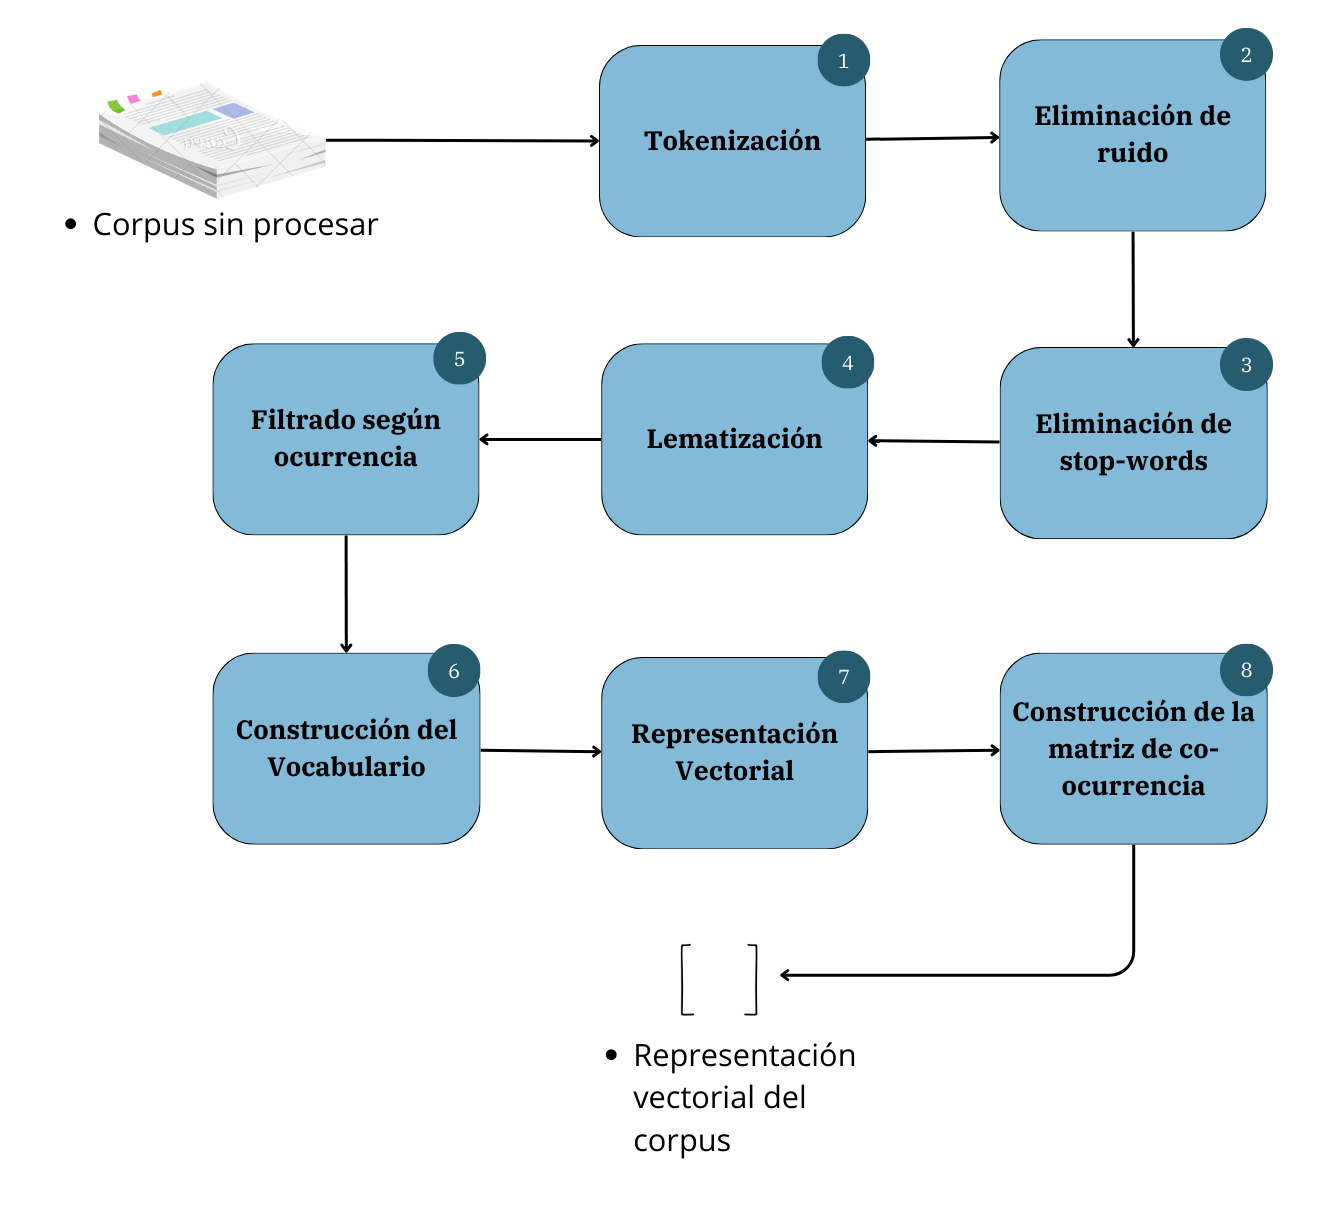
\includegraphics[width=12cm]{lexical_prep}
	\caption{Pre-procesamiento l\'exico}
\end{figure}

\subsection{Identificación de la Cantidad de Tópicos}

Con el objetivo de identificar la cantidad de tópicos presentes en el corpus se propone un enfoque basado en la agrupación semántica de palabras, representadas por sus embeddings (ver figura 2.3). La hip\'otesis es que la cantidad de grupos formados, cada uno con una cantidad suficiente de palabras, proporcionará un indicador de la cantidad de tópicos presentes en el corpus. El algoritmo propuesto se basa en que las palabras que comparten significados similares o co-ocurren con frecuencia en documentos estarán asociadas en conjuntos semánticos, revelando así la presencia de tópicos específicos. Al realizar una agrupación flexible  en el modelo, donde cada palabra puede pertenecer a varios grupos, se refleja la polisemia y la complejidad semántica del lenguaje. 

\begin{figure}[H]
	\centering
	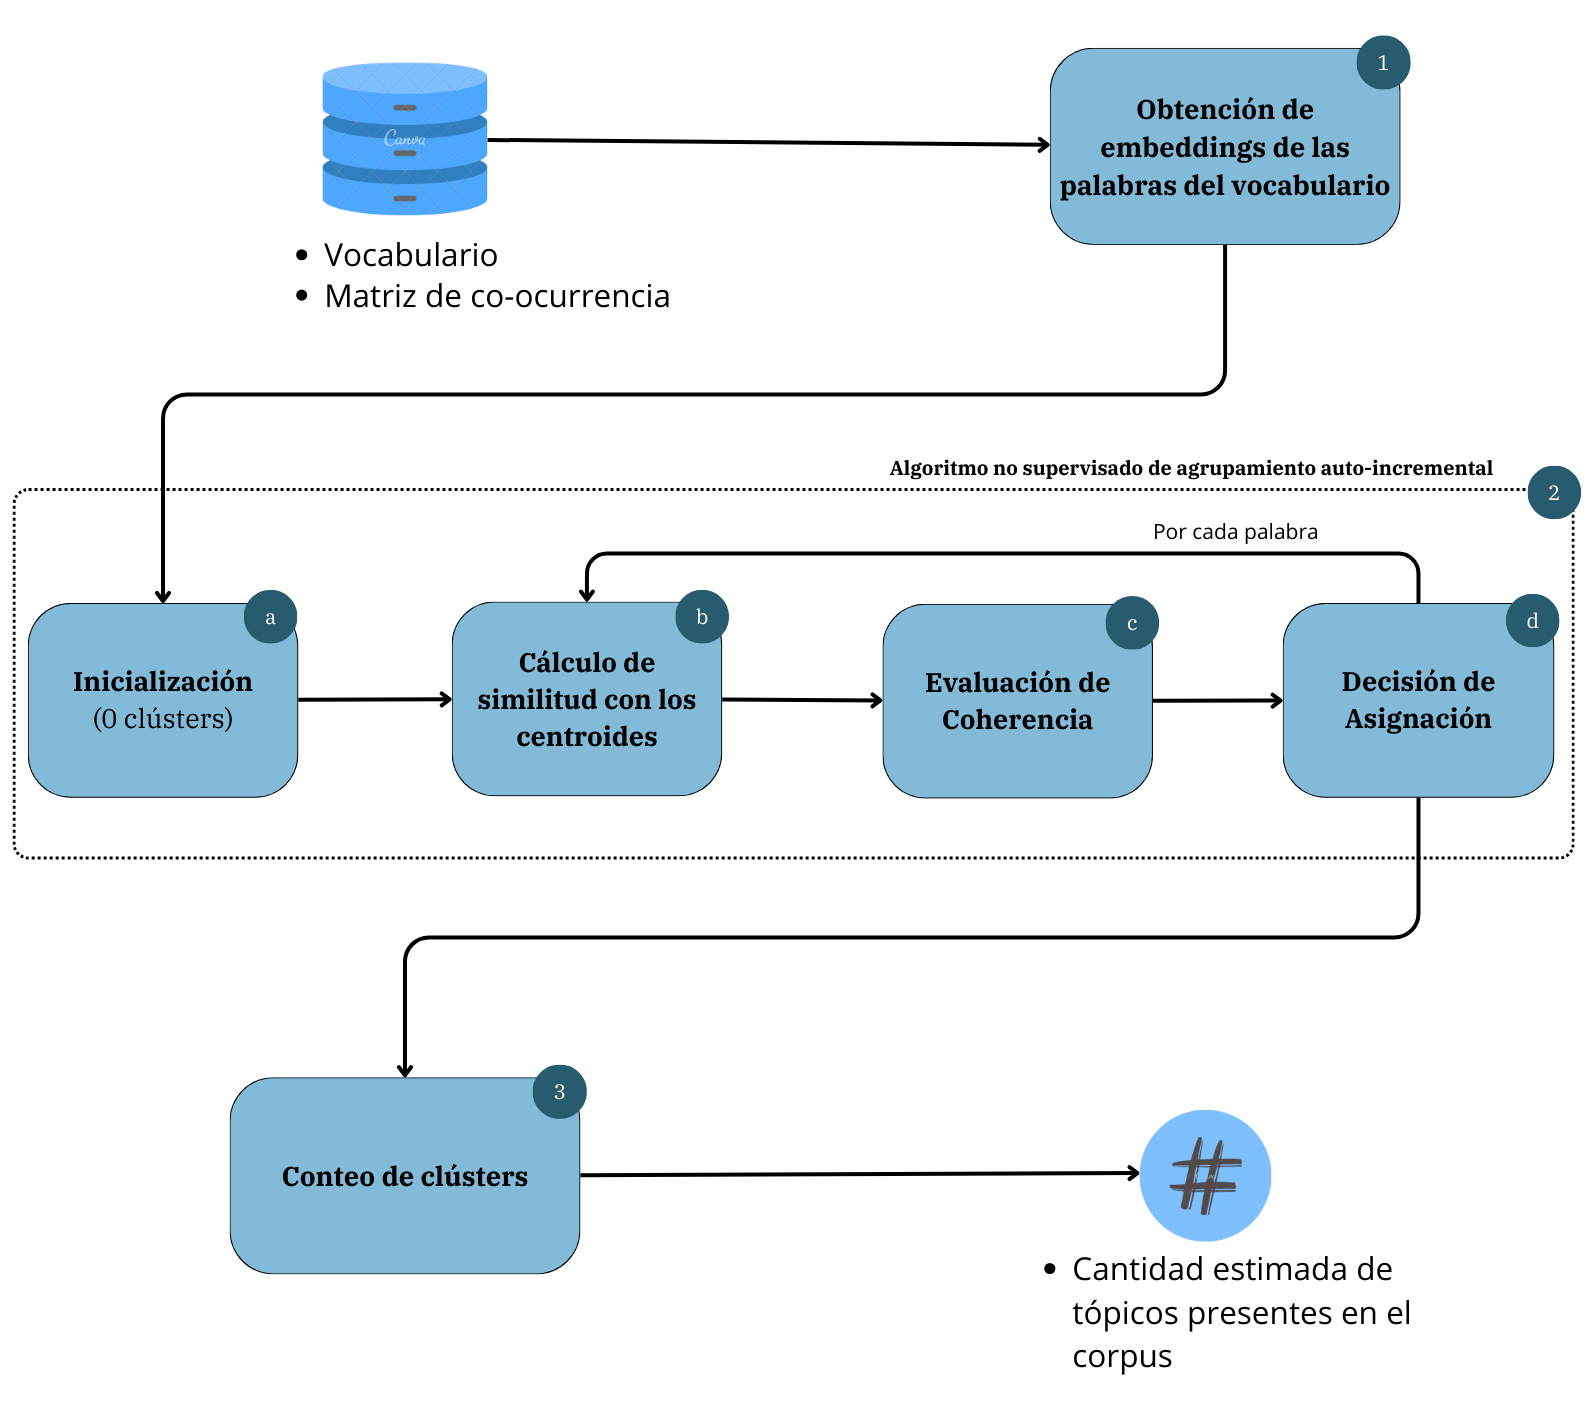
\includegraphics[width=15cm]{k_estimation}
	\caption{Identificaci\'on de la cantidad de t\'opicos}
\end{figure}

En la fase inicial del proceso, se obtienen los embeddings para las palabras que conforman el vocabulario. Para llevar a cabo este propósito, se emplea un modelo preentrenado con extensas cantidades de texto conocido como Google Word2Vec. Este modelo asigna a cada palabra un vector numérico en un espacio multidimensional. Este espacio está diseñado de tal manera que palabras con significados similares tienen representaciones cercanas. De este modo, cada palabra en el vocabulario se vincula a su correspondiente vector semántico, el cual se utilizará posteriormente en el análisis consecuente. Se escogi\'o este espec\'ificamente que es un modelo de dominio general lo cual contribuye a la adaptabilidad del sistema a diferentes contextos. 

En la segunda etapa del proceso de identificación de tópicos, se implementa un algoritmo de agrupamiento autoincremental sobre los embeddings de palabras obtenidos. A diferencia de los métodos convencionales que requieren una predefinición del número de grupos, este enfoque comienza con 0 grupos y estos se construyen dinámicamente a medida que es necesario.

La similitud semántica, basada en la proximidad en el espacio vectorial, desempeña un papel esencial en la creación de grupos al agrupar palabras con significados similares. Sin embargo, los embeddings, debido a su entrenamiento centrado en co-ocurrencias locales, carecen de información contextual más amplia y no logran distinguir entre las diferentes acepciones de una palabra en distintos contextos. Esta limitación puede resultar en la agrupación errónea de palabras con significado compartido pero usos contextuales diferentes. Para superar este desafío, el enfoque propuesto incorpora la matriz de co-ocurrencia del corpus, enriqueciendo la representación al capturar relaciones contextuales entre palabras. Esta integración mejora la precisión y significado en la formación de grupos.

El algoritmo evalúa la similitud entre el embedding a agregar y los centroides de los grupos, seleccionando aquellos cuya similitud sea igual o superior al umbral especificado. Si el vector no cumple con esta medida para ningún grupo existente, se crea uno nuevo. En caso contrario, se analiza la coherencia contextual con las palabras de cada grupo seleccionado, incorporándolo a aquellos en los que al menos la mitad de las palabras sean coherentes con el vector. Este proceso garantiza que las palabras con significados y contextos afines se agrupen de manera coherente.

En la etapa final, se cuentan los grupos con una cardinalidad superior a un umbral predefinido, que representa la cantidad mínima de palabras necesarias para que un grupo sea considerado como un tema. Esta contabilización proporciona una estimación de la cantidad de tópicos presentes en el corpus.

\subsection{Descubrimiento de t\'opicos}

La aplicación de modelos de tópicos desempeña un papel fundamental en el descubrimiento de patrones temáticos en grandes conjuntos de datos textuales. Estos modelos proveen una herramienta eficaz para organizar documentos relacionados y revelar las estructuras temáticas subyacentes en un corpus, facilitando así la extracción de información significativa.

Dentro de este contexto, destaca el algoritmo Latent Dirichlet Allocation (LDA), el asigna palabras a tópicos en documentos, utilizando un proceso probabilístico iterativo. Esto facilita la organización y análisis de grandes conjuntos de datos de texto al proporcionar distribuciones que describen la probabilidad de pertenencia de un documento a un tópico y la asociación de una palabra a un tópico específico.
A pesar de la existencia de enfoques más complejos, la robustez, aplicabilidad general y estatus clásico de LDA, así como su amplia adopción en la literatura especializada, respaldan su confiabilidad. Esto lo posiciona como una elección sólida en el continuo desarrollo y mejora de modelos de tópicos para el descubrimiento temático.

\subsection{Asignaci\'on de nombres a t\'opicos}

En el ámbito del análisis de tópicos, conferir nombres de manera automática a los t\'opicos identificados no solo añade claridad interpretativa, sino que también facilita la comprensión y exploración de grandes conjuntos de documentos. Este proceso, esencial para dotar de significado a los patrones temáticos descubiertos, se llevará a cabo mediante la utilización de una ontología de dominio general. Al aprovechar la riqueza semántica y la estructura jerárquica de esta ontología, se busca lograr una asignación de nombres precisa y contextualizada para cada tópico identificado. Este enfoque (ver figura 2.4) contribuirá a mejorar la interpretabilidad y utilidad de los resultados obtenidos en la fase de descubrimiento de tópicos mediante Latent Dirichlet Allocation (LDA).

\begin{figure}[H]
	\centering
	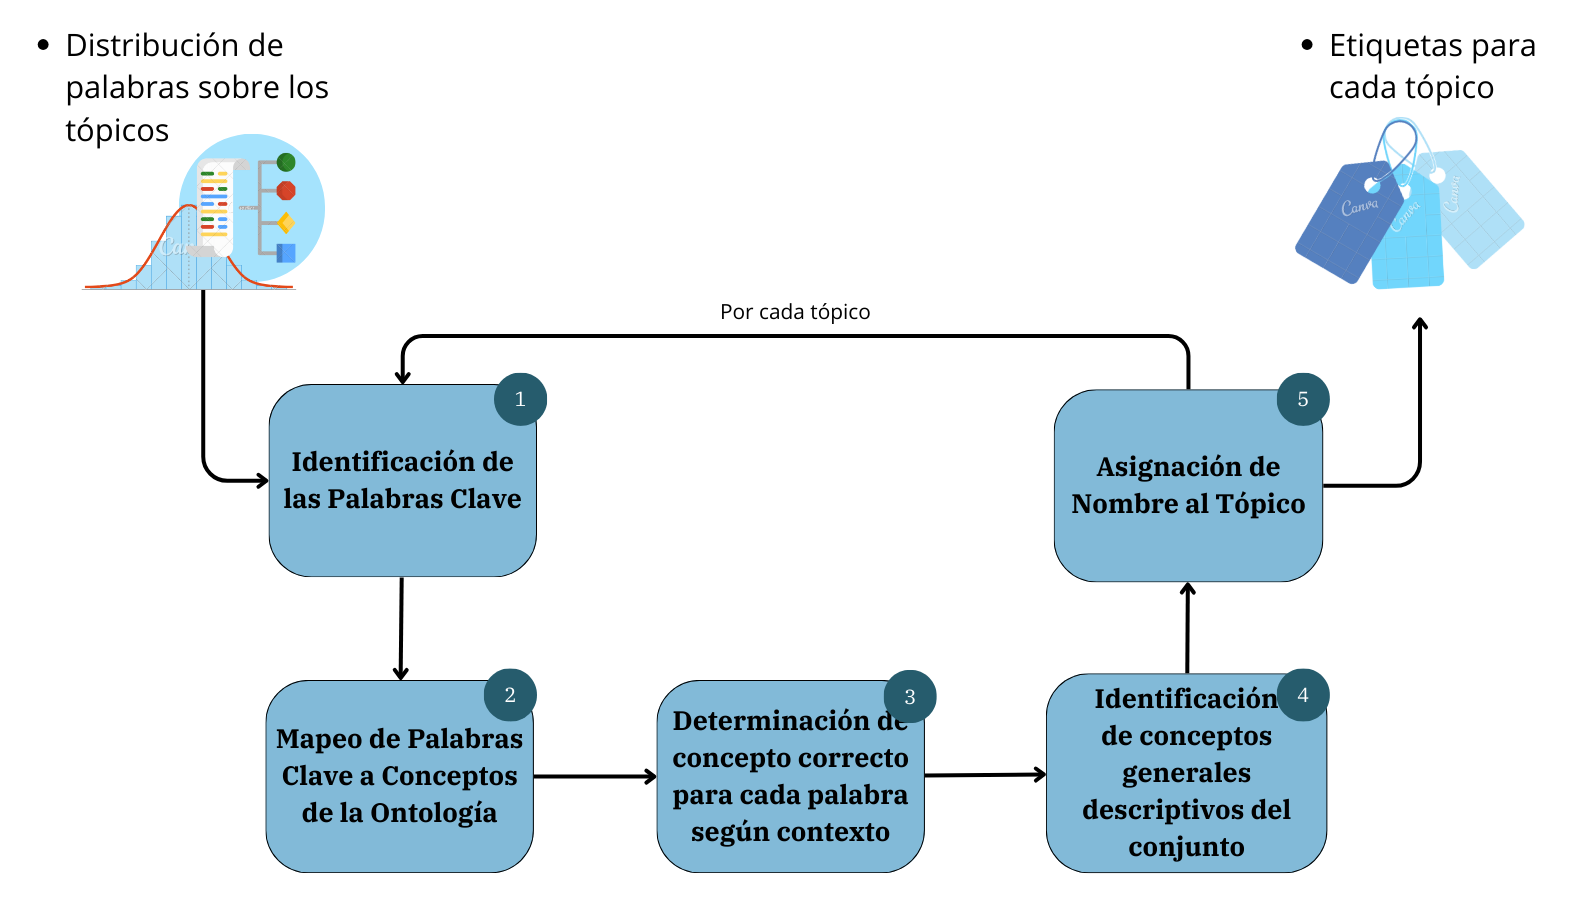
\includegraphics[width=15cm]{topic_naming}
	\caption{Asignaci\'on de nombres a t\'opicos}
\end{figure}

En la primera etapa, se seleccionan las palabras más probables para cada tópico a partir de las probabilidades proporcionadas por el modelo LDA. Este proceso incluye la aplicación de un umbral específico, lo que permite identificar de manera efectiva las palabras clave más representativas de cada temática. Estas palabras clave serán la base para la posterior asignación de nombres a los tópicos. Luego, cada palabra clave seleccionada se asigna a los conceptos pertinentes presentes en la ontología de dominio general. Es importante tener en cuenta que las ontologías están diseñadas para abordar la polisemia del lenguaje natural, lo que significa que, en la mayoría de los casos, una palabra puede estar asociada a más de un concepto en la ontología.

Luego, se hace necesario en la siguiente etapa, seleccionar el concepto adecuado para cada palabra de acuerdo con el contexto en el que aparece en el corpus. Con este prop\'osito se aplican técnicas de Disambiguación del Sentido de las Palabras (WSD, por sus siglas en inglés). Este paso es fundamental para garantizar una asignación precisa y contextualizada de conceptos ontológicos que engloben a las palabras clave identificadas en los tópicos. Se exploran tres variantes para abordar este desafío.

La primera variante representa una mejora significativa sobre el algoritmo tradicional de Lesk utilizado en WSD. Mientras que el algoritmo de Lesk convencional se basa en coincidencias exactas entre las palabras del contexto y las presentes en las definiciones de los sentidos, la variante propuesta supera esta limitación. El enfoque propuesto aprovecha embeddings de palabras para capturar la semántica y el significado contextual de las palabras, calculando la media de los embeddings del contexto. Además, para cada definición en la ontología, se calcula la media aritm\'etica de los embeddings de las palabras asociadas a esa definición. La elección de la definición adecuada se realiza comparando las medias de embeddings. Se selecciona la definición cuya media de embeddings se aproxima más al contexto en términos de similitud del coseno. De esta forma se permite una mayor flexibilidad y capacidad para capturar relaciones semánticas más sutiles, mejorando así la precisión y el rendimiento del algoritmo en tareas de WSD.

Este problema de WSD se puede abordar tambi\'en como un problema de optimizaci\'on. Se plantea como la tarea de seleccionar, de una lista de n elementos (palabras), cada uno asociado a k características (definiciones), con k variable, n características exactamente, de modo que se maximice la similitud entre cada par de características seleccionadas. En este contexto, maximizar la similitud equivale a minimizar el camino entre dos definiciones en la ontolog\'ia. Para resolver esta tarea, se utiliza el algoritmo Simplex y se concibe un algoritmo genético, permitiendo así encontrar la mejor combinación de conceptos ontológicos asociados a las palabras clave en los tópicos identificados. Este enfoque optimizado pretende mejorar la precisión en la asignación de conceptos y contribuir a una representación semántica más refinada de los tópicos en el contexto ontológico.

Una vez se haya seleccionado la definici\'on correcta en la ontología para cada palabra clave, se procede a identificar los conceptos más generales asociados a cada una. Se busca construir una lista de conceptos generales para cada palabra y, posteriormente, se aplica una función de peso híbrida para determinar cu\'ales de estos conceptos describen mejor al grupo de palabras. Esta función de peso considera diversos factores para evaluar la relevancia de cada concepto general. Entre los factores se encuentran: la pofundidad en la jerarquía de la ontología, indicando cuán específico es el concepto, la información de contenido para obtener contexto, la similitud con las palabras presentes en el contexto y la generalidad del concepto. La función de peso híbrida permite asignar una puntuación a cada concepto general, tomando en cuenta la combinación de estos factores. Finalmente, se toman los conceptos generales que han obtenido la puntuación más alta, lo que asegura una selección de los términos más adecuados y representativos para denominar los tópicos identificados. Este enfoque garantiza una asignación de nombres que considere tanto la estructura jerárquica de la ontología como la riqueza semántica del contexto circundante.

\section{Recuperaci\'on por t\'opicos}

En esta sección se aborda el dise\~no de un motor de búsqueda basado en modelos el modelo propuesto anteriormente. El propósito principal de este desarrollo es aprovechar los resultados obtenidos en la etapa anterior para mejorar y la eficiencia y visualizaci\'on de los resultados en la exploraci\'on.

Esta etapa se inicia con la recepción de consultas por parte de los usuarios. Utilizando el modelo de tópicos LDA previamente entrenado, se identifican los tópicos más relevantes para la consulta. Posteriormente, se lleva a cabo un filtrado de documentos asociados a tópicos no relevantes para la consulta, mejorando significativamente la eficiencia del sistema al centrar la búsqueda únicamente en la información contextualmente relacionada con los temas de interés del usuario. Se calcula la similitud entre los documentos de los t\'opicos relevantes y la consulta, y se presentan los resultados al usuario ordenados segun su relevancia, por t\'opicos. 

